\documentclass[12pt,a4paper]{article}

% ─── Page Layout ───────────────────────────────────────────────────────────────
\usepackage[a4paper, margin=0.8in, headheight=14pt]{geometry}

% ─── Fonts (XeLaTeX) ───────────────────────────────────────────────────────────
\usepackage{fontspec}
\usepackage{unicode-math}
\setmainfont{TeX Gyre Pagella}
\setmonofont[Scale=0.88]{TeX Gyre Cursor}
\setmathfont{Latin Modern Math}

% ─── Packages ──────────────────────────────────────────────────────────────────
\usepackage{xcolor}
\usepackage{colortbl}
\usepackage{titlesec}
\usepackage{enumitem}
\usepackage{tabularx}
\usepackage{booktabs}
\usepackage{array}
\usepackage{amsmath}
\usepackage{tikz}
\usetikzlibrary{shapes.geometric, arrows.meta, positioning, calc, fit, decorations.pathreplacing, decorations.pathmorphing}
\usepackage{tcolorbox}
\tcbuselibrary{skins, breakable}
\usepackage{hyperref}
\usepackage{fancyhdr}
\usepackage{graphicx}
\usepackage{microtype}
\hyphenpenalty=10000
\exhyphenpenalty=10000
\sloppy
\usepackage{caption}
\usepackage{setspace}
\usepackage{multirow}
\usepackage{tocloft}

% ─── Q&A helper ────────────────────────────────────────────────────────────────
\newcommand{\Q}[1]{\textbf{#1}\par\noindent\ignorespaces}

% ─── Colour Palette ────────────────────────────────────────────────────────────
\definecolor{myred}{RGB}{196,30,58}
\definecolor{mydark}{RGB}{30,30,50}
\definecolor{mygreen}{RGB}{14,120,80}
\definecolor{myteal}{RGB}{0,130,140}
\definecolor{myamber}{RGB}{180,100,0}
\definecolor{mypurple}{RGB}{100,30,160}
\definecolor{mygray}{RGB}{246,247,249}
\definecolor{mgframe}{RGB}{180,185,200}
\definecolor{watermark}{RGB}{145,150,170}
\definecolor{hdrred}{RGB}{250,232,235}
\definecolor{hdrgreen}{RGB}{220,244,233}
\definecolor{hdrteal}{RGB}{220,242,244}
\definecolor{hdramber}{RGB}{253,242,215}
\definecolor{hdrpurple}{RGB}{238,228,255}
\definecolor{hdrgray}{RGB}{238,240,245}
\definecolor{rowalt}{RGB}{250,251,253}

% ─── Section Formatting ────────────────────────────────────────────────────────
\titleformat{\section}
  {\large\bfseries\color{myred}}{\thesection.}{0.5em}{}
  [\vspace{1pt}{\color{myred}\rule{\linewidth}{0.8pt}}]
\titleformat{\subsection}
  {\normalsize\bfseries\color{myteal}}{\thesubsection}{0.5em}{}
\titlespacing*{\section}{0pt}{18pt}{7pt}
\titlespacing*{\subsection}{0pt}{11pt}{4pt}

% ─── Paragraph ─────────────────────────────────────────────────────────────────
\setlength{\parindent}{0pt}
\setlength{\parskip}{4pt}

% ─── TOC Styling ───────────────────────────────────────────────────────────────
\renewcommand{\cfttoctitlefont}{\large\bfseries\color{myred}}
\renewcommand{\cftaftertoctitle}{\par\noindent{\color{myred}\rule{\linewidth}{0.8pt}}}
\setlength{\cftbeforetoctitleskip}{0pt}
\setlength{\cftaftertoctitleskip}{6pt}
\renewcommand{\cftsecfont}{\normalsize\bfseries\color{mydark}}
\renewcommand{\cftsecpagefont}{\normalsize\bfseries\color{mydark}}
\renewcommand{\cftsecleader}{\cftdotfill{\cftdotsep}}
\setlength{\cftbeforesecskip}{7pt}
\renewcommand{\cftsubsecfont}{\small\color{mydark}}
\renewcommand{\cftsubsecpagefont}{\small\color{mydark}}
\setlength{\cftbeforesubsecskip}{3pt}
\setlength{\cftsubsecindent}{1.4em}

% ─── Table helpers ─────────────────────────────────────────────────────────────
\renewcommand{\arraystretch}{1.45}
\setlength{\tabcolsep}{6pt}
\arrayrulecolor{mydark}
\newcolumntype{B}[1]{>{\small\bfseries\raggedright\arraybackslash}m{#1}}
\newcolumntype{C}[1]{>{\centering\arraybackslash}m{#1}}
\newcolumntype{Y}{>{\small\raggedright\arraybackslash}X}
\renewcommand{\tabularxcolumn}[1]{m{#1}}

% ─── Header / Footer ───────────────────────────────────────────────────────────
\pagestyle{fancy}
\fancyhf{}
\fancyhead[L]{\small\color{myred}\textbf{OE-EC704A}\;\color{mydark}--- Web Technology}
\fancyhead[R]{\small\color{myteal}\textbf{Module 1 Notes}}
\fancyfoot[C]{\small\color{mydark}\thepage}
\fancyfoot[R]{\small\color{watermark}\textit{\copyright\ Biraj}}
\renewcommand{\headrulewidth}{0.5pt}
\renewcommand{\footrulewidth}{0.3pt}

% ─── Hyperref ──────────────────────────────────────────────────────────────────
\hypersetup{
  colorlinks=true, linkcolor=myteal, urlcolor=myteal,
  pdfauthor={Biraj Sarkar},
  pdftitle={OE-EC704A --- Module 1 Notes}
}

% ─── tcolorbox styles ──────────────────────────────────────────────────────────
\tcbset{
  tikzbox/.style={
    colback=mygray, colframe=mgframe, boxrule=0.6pt, arc=4pt,
    left=8pt, right=8pt, top=6pt, bottom=6pt,
    colbacktitle=mgframe, coltitle=mydark,
    fonttitle=\small\bfseries
  },
  defbox/.style={
    colback=hdrgreen, colframe=mygreen, boxrule=0.8pt, arc=4pt,
    left=9pt, right=9pt, top=6pt, bottom=6pt,
    colbacktitle=mygreen, coltitle=white,
    fonttitle=\small\bfseries
  },
  formulabox/.style={
    colback=hdrteal, colframe=myteal, boxrule=0.8pt, arc=4pt,
    left=9pt, right=9pt, top=7pt, bottom=7pt,
    colbacktitle=myteal, coltitle=white,
    fonttitle=\small\bfseries
  },
  examplebox/.style={
    colback=hdramber, colframe=myamber, boxrule=0.8pt, arc=4pt,
    left=9pt, right=9pt, top=6pt, bottom=6pt,
    colbacktitle=myamber, coltitle=white,
    fonttitle=\small\bfseries
  },
  masonbox/.style={
    colback=hdrpurple, colframe=mypurple, boxrule=0.8pt, arc=4pt,
    left=9pt, right=9pt, top=6pt, bottom=6pt,
    colbacktitle=mypurple, coltitle=white,
    fonttitle=\small\bfseries
  },
  exambox/.style={
    colback=hdrpurple, colframe=mypurple, boxrule=1pt, arc=5pt,
    left=10pt, right=10pt, top=8pt, bottom=8pt,
    colbacktitle=mypurple, coltitle=white,
    fonttitle=\bfseries,
    breakable, title after break={\textbf{Frequently Asked / Viva Questions (contd.)}}}
}
\tcbset{breakable}

% ─── TikZ styles ───────────────────────────────────────────────────────────────
\tikzset{
  block/.style={rectangle, draw=myteal, fill=hdrteal,
    text width=2.5cm, align=center, minimum height=1.0cm,
    font=\small, rounded corners=3pt, line width=0.7pt},
  redblock/.style={rectangle, draw=myred, fill=hdrred,
    text width=2.5cm, align=center, minimum height=1.0cm,
    font=\small, rounded corners=3pt, line width=0.7pt},
  netnode/.style={rectangle, draw=myteal, fill=hdrteal,
    text width=1.8cm, align=center, minimum height=0.8cm,
    font=\small, rounded corners=3pt, line width=0.7pt},
  sumjunc/.style={circle, draw=myamber, fill=hdramber,
    minimum size=0.6cm, font=\small, line width=0.8pt},
  snode/.style={circle, draw=mypurple, fill=hdrpurple,
    minimum size=0.55cm, font=\footnotesize, line width=0.7pt},
  arrow/.style={-Stealth, thick, color=mydark},
  redarrow/.style={-Stealth, thick, color=myred},
  line/.style={thick, color=mydark}
}

% ═══════════════════════════════════════════════════════════════════════════════
\begin{document}
% ═══════════════════════════════════════════════════════════════════════════════

\begin{center}
  {\LARGE\bfseries\color{myred} OE-EC704A --- Web Technology}\\[5pt]
  {\normalsize\color{mydark} Semester VII \quad$\bullet$\quad 3L:0T:0P \quad$\bullet$\quad 3 Credits}\\[3pt]
  {\normalsize\color{myteal}\textbf{Module 1 Exam Notes: Web Development Basics (HTML \& CSS)}}\\[3pt]
  {\small\color{mydark} CGEC \;$|$\; B.Tech ECE (2023--27) \;$|$\; \textit{Biraj Sarkar}}
\end{center}
\vspace{2pt}
\noindent{\color{myred}\rule{\linewidth}{1.5pt}}
\vspace{2pt}

\hypersetup{linkcolor=mydark}
\tableofcontents
\hypersetup{linkcolor=myteal}
\newpage

% ===============================================================================
\section{Introduction to Web Development Basics}
% ===============================================================================

Modern web development relies on a client-server architecture. Web pages are hosted on web servers and requested by clients (web browsers) via HTTP/HTTPS protocols.

\begin{tcolorbox}[defbox, title={\textbf{Client-Server Web Architecture}}]
The \textbf{Client-Server Model} is a distributed application structure that partitions tasks between resource providers (\textbf{servers}) and service requesters (\textbf{clients}). In web technology:
\begin{itemize}[leftmargin=*, itemsep=3pt]
  \item \textbf{Client (Web Browser):} Sends HTTP requests, parses HTML/CSS/JS, and renders the user interface.
  \item \textbf{Server (Web Server):} Listens for incoming requests on ports 80 (HTTP) or 443 (HTTPS), processes logic, and returns the requested resources.
\end{itemize}
\end{tcolorbox}

\begin{tcolorbox}[tikzbox, title={Web Architecture: Client-Server Flow}]
\centering
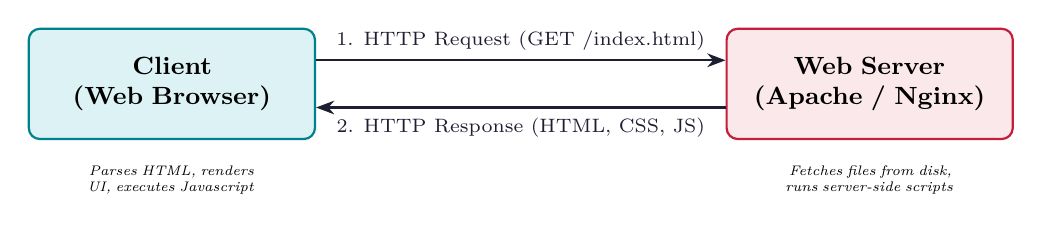
\begin{tikzpicture}[node distance=1.5cm and 5.2cm,
  browser/.style={rectangle, draw=myteal, fill=hdrteal, text width=3.4cm,
    align=center, minimum height=1.4cm, font=\small\bfseries, rounded corners=4pt, line width=0.8pt},
  server/.style={rectangle, draw=myred, fill=hdrred, text width=3.4cm,
    align=center, minimum height=1.4cm, font=\small\bfseries, rounded corners=4pt, line width=0.8pt}]

  % Nodes
  \node[browser] (client) {Client\\(Web Browser)};
  \node[server, right=of client] (server) {Web Server\\(Apache / Nginx)};

  % Paths
  \draw[arrow, transform canvas={yshift=0.3cm}] (client) -- (server) 
    node[midway, above, font=\scriptsize] {1. HTTP Request (GET /index.html)};
  \draw[arrow, transform canvas={yshift=-0.3cm}] (server) -- (client) 
    node[midway, below, font=\scriptsize] {2. HTTP Response (HTML, CSS, JS)};
    
  % Explanations
  \node[below=0.2cm of client, font=\tiny\itshape, text width=3.4cm, align=center] {Parses HTML, renders UI, executes Javascript};
  \node[below=0.2cm of server, font=\tiny\itshape, text width=3.4cm, align=center] {Fetches files from disk, runs server-side scripts};
\end{tikzpicture}
\end{tcolorbox}

\subsection{HTML vs. XML}
HTML and XML are both markup languages based on SGML, but they serve fundamentally different purposes:

\par\noindent
{\renewcommand{\arraystretch}{1.5}%
\begin{tabularx}{\linewidth}{|B{3.5cm}|Y|Y|}
\hline
\textbf{Feature} & \textbf{HTML (HyperText Markup Language)} & \textbf{XML (eXtensible Markup Language)} \\
\hline
\textbf{Primary Purpose} & Displaying and formatting data to users. & Transporting, storing, and structuring data. \\
\hline
\textbf{Tags} & Predefined tags (e.g., \texttt{<html>}, \texttt{<p>}). & Custom/user-defined tags based on data. \\
\hline
\textbf{Syntax Strictness} & Forgiving (errors don't crash rendering). & Extremely strict (well-formed check required). \\
\hline
\textbf{Case Sensitivity} & Case-insensitive (\texttt{<DIV>} and \texttt{<div>}). & Strictly case-sensitive. \\
\hline
\textbf{Closing Tags} & Optional for some tags (e.g., \texttt{<img>}, \texttt{<br>}). & Mandatory for all tags. \\
\hline
\end{tabularx}}

% ===============================================================================
\section{HTML Basics and Document Structure}
% ===============================================================================

\begin{tcolorbox}[defbox, title={\textbf{HTML --- HyperText Markup Language}}]
\textbf{HTML} is the standard markup language used to create the structure of web pages. It uses a set of hierarchical elements represented by tags to organize headings, paragraphs, tables, images, and other media elements.
\end{tcolorbox}

\subsection{Standard Skeleton of an HTML5 Document}
Every HTML document must follow a standard structural hierarchy:
\begin{spacing}{1.0}
\begin{verbatim}
<!DOCTYPE html>
<html>
  <head>
    <meta charset="UTF-8">
    <title>My Web Page</title>
  </head>
  <body>
    <h1>Welcome to Web Technology</h1>
    <p>This is a paragraph.</p>
  </body>
</html>
\end{verbatim}
\end{spacing}

\begin{tcolorbox}[tikzbox, title={HTML Document Object Model (DOM) Tree}]
\centering
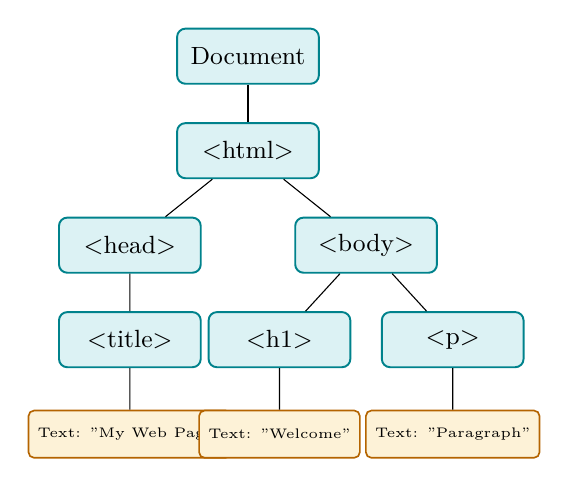
\begin{tikzpicture}[
  level 1/.style={sibling distance=5cm, level distance=1.2cm},
  level 2/.style={sibling distance=3cm, level distance=1.2cm},
  level 3/.style={sibling distance=2.2cm, level distance=1.2cm},
  node/.style={rectangle, draw=myteal, fill=hdrteal, minimum height=0.7cm, minimum width=1.8cm, font=\small, rounded corners=3pt, align=center, line width=0.7pt},
  textnode/.style={rectangle, draw=myamber, fill=hdramber, minimum height=0.6cm, minimum width=1.6cm, font=\tiny, rounded corners=2pt, align=center, line width=0.6pt}
]
  \node[node] {Document}
    child { node[node] {<html>}
      child { node[node] {<head>}
        child { node[node] {<title>}
          child { node[textnode] {Text: "My Web Page"} }
        }
      }
      child { node[node] {<body>}
        child { node[node] {<h1>}
          child { node[textnode] {Text: "Welcome"} }
        }
        child { node[node] {<p>}
          child { node[textnode] {Text: "Paragraph"} }
        }
      }
    };
\end{tikzpicture}
\end{tcolorbox}

\subsection{Block-level vs. Inline Elements}
HTML elements are categorized based on their default layout behaviors:

\par\noindent
{\renewcommand{\arraystretch}{1.5}%
\begin{tabularx}{\linewidth}{|B{3.2cm}|Y|Y|}
\hline
\textbf{Feature} & \textbf{Block-level Elements} & \textbf{Inline Elements} \\
\hline
\textbf{Layout Behavior} & Starts on a new line and takes up full width. & Stays on the same line and occupies only needed width. \\
\hline
\textbf{Margins \& Padding} & Fully respected on all four sides. & Top and bottom margins are ignored. \\
\hline
\textbf{Containment} & Can contain block or inline elements. & Can only contain inline elements / text. \\
\hline
\textbf{Examples} & \texttt{<div>, <p>, <h1>-<h6>, <ul>, <ol>, <table>} & \texttt{<span>, <a>, <strong>, <em>, <img>, <input>} \\
\hline
\end{tabularx}}

\subsection{Essential HTML Components}

\textbf{1. Lists:} HTML supports three list types:
\begin{itemize}[leftmargin=*, itemsep=3pt]
  \item \textbf{Unordered List (\texttt{<ul>}):} Bulleted list items using the \texttt{<li>} tag.
  \item \textbf{Ordered List (\texttt{<ol>}):} Numbered list items with customizable types (numeric, alphabetic, roman).
  \item \textbf{Description List (\texttt{<dl>}):} Pairs of terms (\texttt{<dt>}) and descriptions (\texttt{<dd>}).
\end{itemize}

\textbf{2. Links (Anchors \texttt{<a>}):} Used for navigating between pages or sections:
\begin{itemize}[leftmargin=*, itemsep=3pt]
  \item \textbf{Absolute Link:} Links to a fully qualified URL (e.g., \texttt{href="https://google.com"}).
  \item \textbf{Relative Link:} Links to a local resource relative to the file path (e.g., \texttt{href="about.html"}).
  \item \textbf{Email Link:} Triggers the client's email client using the mailto protocol (e.g., \texttt{href="mailto:test@test.com"}).
  \item \textbf{Anchor Targets:} Uses \texttt{target="\_blank"} to open in a new tab or \texttt{target="\_self"} for the same frame.
\end{itemize}

\textbf{3. Tables (\texttt{<table>}):} Formats data in rows and columns:
\begin{itemize}[leftmargin=*, itemsep=3pt]
  \item \textbf{Rowspan:} Extends a cell vertically across multiple rows (e.g., \texttt{<td rowspan="2">}).
  \item \textbf{Colspan:} Extends a cell horizontally across multiple columns (e.g., \texttt{<td colspan="3">}).
\end{itemize}

\textbf{4. Forms (\texttt{<form>}):} Captures and submits user inputs to a server. Key attributes:
\begin{itemize}[leftmargin=*, itemsep=3pt]
  \item \textbf{action:} The URL of the server-side endpoint that handles the submitted form data.
  \item \textbf{method:} The HTTP method used to send data (\texttt{GET} or \texttt{POST}).
  \item \textbf{Input Types:} Text, password, radio buttons, checkboxes, email, submit, file, number.
\end{itemize}

\textbf{5. Frames (\texttt{<frameset>}, \texttt{<frame>}, \texttt{<iframe>}):} Used to split the browser window into multiple independent document spaces:
\begin{itemize}[leftmargin=*, itemsep=3pt]
  \item \textbf{Traditional Frameset (\texttt{<frameset>}):} Replaces the \texttt{<body>} tag in HTML4 to partition the screen layout into rows or columns (e.g., \texttt{<frameset cols="25\%, 75\%">}). Each partition is defined using a \texttt{<frame src="...">} tag. \textit{Note: Deprecated in HTML5 due to poor accessibility, bookmarking difficulties, and bad SEO indexing.}
  \item \textbf{Inline Frames (\texttt{<iframe>}):} Used inside a standard \texttt{<body>} tag to embed another HTML page within the current page (e.g., \texttt{<iframe src="inner.html" width="300" height="200"></iframe>}). Widely used for embedding maps, videos, and third-party widgets.
\end{itemize}

% ===============================================================================
\section{CSS (Cascading Style Sheets)}
% ===============================================================================

\begin{tcolorbox}[defbox, title={\textbf{CSS --- Cascading Style Sheets}}]
\textbf{CSS} is a style sheet language used to describe the presentation, design, formatting, and layout of a document written in HTML. It separates structure from style, allowing consistent look-and-feel across multiple web pages.
\end{tcolorbox}

\subsection{Types of CSS Integration}

\par\noindent
{\renewcommand{\arraystretch}{1.5}%
\begin{tabularx}{\linewidth}{|B{3.0cm}|Y|Y|Y|}
\hline
\textbf{CSS Type} & \textbf{Syntax Example} & \textbf{Advantages} & \textbf{Disadvantages} \\
\hline
\textbf{Inline CSS} & \texttt{<p style="color:red;">} & High priority; quick overrides. & Messy; violates separation of concerns. \\
\hline
\textbf{Internal CSS} & \texttt{<style> p \{ color: red; \} </style>} & Contained inside single page; no extra HTTP request. & Reusability limit across multiple pages. \\
\hline
\textbf{External CSS} & \texttt{<link rel="stylesheet" href="style.css">} & High reuse; caching support; clean separation. & Requires extra network HTTP request. \\
\hline
\end{tabularx}}

\subsection{CSS Selectors}
CSS selectors target specific HTML elements for styling:
\begin{itemize}[leftmargin=*, itemsep=3pt]
  \item \textbf{Element Selector:} Targets all elements of a type (e.g., \texttt{p \{ color: red; \}}).
  \item \textbf{Class Selector:} Targets elements with a matching class name, preceded by a dot (e.g., \texttt{.container \{ width: 80\%; \}}).
  \item \textbf{ID Selector:} Targets a single element with a matching ID, preceded by a hash (e.g., \texttt{\#header \{ height: 60px; \}}). ID must be unique within the page.
  \item \textbf{Universal Selector:} Targets every element in the DOM using asterisk (e.g., \texttt{* \{ margin: 0; \}}).
\end{itemize}

\subsection{The CSS Box Model}
Every element in HTML is rendered as a rectangular box. The CSS Box Model defines how the size and spacing of this box are calculated.

\begin{tcolorbox}[tikzbox, title={CSS Box Model Layout}]
\centering
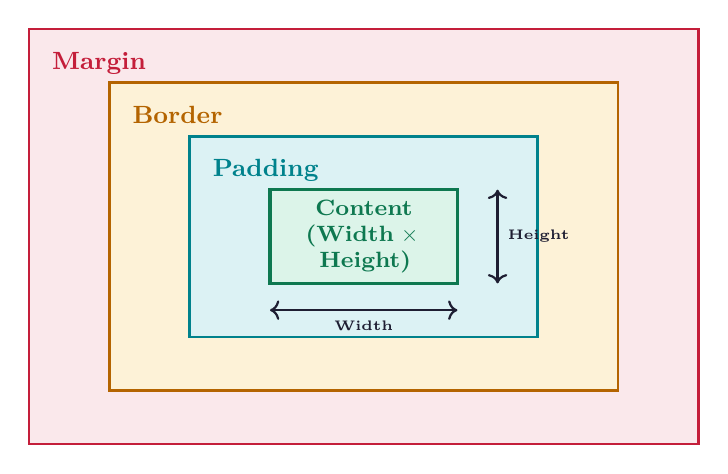
\begin{tikzpicture}[scale=0.85]
  % Outermost Margin
  \draw[line, fill=hdrred, draw=myred, line width=1pt] (0,0) rectangle (10,6.2);
  \node[anchor=north west, color=myred, font=\small\bfseries] at (0.2, 6.0) {Margin};

  % Border
  \draw[line, fill=hdramber, draw=myamber, line width=1pt] (1.2,0.8) rectangle (8.8,5.4);
  \node[anchor=north west, color=myamber, font=\small\bfseries] at (1.4, 5.2) {Border};

  % Padding
  \draw[line, fill=hdrteal, draw=myteal, line width=1pt] (2.4,1.6) rectangle (7.6,4.6);
  \node[anchor=north west, color=myteal, font=\small\bfseries] at (2.6, 4.4) {Padding};

  % Content
  \draw[line, fill=hdrgreen, draw=mygreen, line width=1.2pt] (3.6,2.4) rectangle (6.4,3.8);
  \node[color=mygreen, font=\footnotesize\bfseries, align=center, text width=2.4cm] at (5,3.1) {Content\\(Width $\times$ Height)};

  % Measurement markers
  \draw[arrow, <->, color=mydark] (3.6, 2.0) -- (6.4, 2.0) node[midway, below, font=\tiny\bfseries] {Width};
  \draw[arrow, <->, color=mydark] (7.0, 2.4) -- (7.0, 3.8) node[midway, right, font=\tiny\bfseries] {Height};
\end{tikzpicture}
\end{tcolorbox}

The dimensions of an element are computed based on the \texttt{box-sizing} property:
\begin{itemize}[leftmargin=*, itemsep=3pt]
  \item \textbf{\texttt{content-box} (Default):} Total Width = $\text{width} + \text{left/right padding} + \text{left/right border} + \text{left/right margin}$.
  \item \textbf{\texttt{border-box}:} Total Width = $\text{width} + \text{left/right margin}$ (padding and border are absorbed inside the specified width).
\end{itemize}

\newpage
% ===============================================================================
\begin{center}
  {\large\bfseries\color{myred} Quick Revision --- Module 1}\\[3pt]
  {\small\color{mydark} Web Development Basics (HTML \& CSS) $|$ OE-EC704A}
\end{center}
\noindent{\color{myred}\rule{\linewidth}{1.2pt}}
\vspace{4pt}

\begin{tcolorbox}[formulabox, title={\textbf{Core HTML Tags \& CSS Syntax}}]
{\renewcommand{\arraystretch}{1.3}%
\begin{tabularx}{\linewidth}{l Y}
\textbf{HTML Form / Tag} & \textbf{Syntax and Key Attributes} \\
\hline
Hyperlink Anchor & \texttt{<a href="URL" target="\_blank">Link Text</a>} \\
Embedded Image & \texttt{<img src="path" alt="Fallback text" width="500">} \\
HTML Table Structure & \texttt{<table> <tr> <td colspan="2">Data</td> </tr> </table>} \\
HTML Form Tag & \texttt{<form action="/login" method="POST"> inputs... </form>} \\
\hline
\textbf{CSS Selector Type} & \textbf{Syntax and Example Usage} \\
\hline
CSS Syntax Rule & \texttt{selector \{ property: value; \}} \\
Class Styling & \texttt{.button \{ background-color: blue; padding: 10px; \}} \\
ID Styling & \texttt{\#main-nav \{ display: flex; justify-content: space-between; \}} \\
Universal Reset & \texttt{* \{ box-sizing: border-box; margin: 0; padding: 0; \}} \\
\end{tabularx}}
\end{tcolorbox}

\begin{tcolorbox}[defbox, title={\textbf{One-Line Definitions}}]
\begin{itemize}[leftmargin=*, itemsep=2pt]
  \item \textbf{HTML:} Structured markup language defining content hierarchy of a web document.
  \item \textbf{CSS:} Style sheet language used for presenting and laying out HTML elements.
  \item \textbf{DOM (Document Object Model):} An API representing an HTML document as a logical tree structure.
  \item \textbf{Tag:} A code marker representing the start or end of an HTML element (e.g., \texttt{<p>}).
  \item \textbf{Element:} A complete component consisting of start tag, content, and end tag.
  \item \textbf{Attribute:} Name-value pairs inside HTML tags that modify their behavior or supply metadata.
  \item \textbf{Viewport:} The visible area of a web page on a client device screen.
  \item \textbf{URL (Uniform Resource Locator):} The global reference address of a web resource on the Internet.
\end{itemize}
\end{tcolorbox}

\begin{tcolorbox}[exambox, title={\textbf{Frequently Asked / Viva Questions}}]
\begin{enumerate}[leftmargin=*, label=\textbf{Q\arabic*.}, itemsep=5pt]
  \item \Q{What is the difference between \texttt{GET} and \texttt{POST} methods in forms?}
        \texttt{GET} appends form data directly to the URL as query parameters, rendering it visible and bookmarkable. It is intended for idempotent requests. \texttt{POST} sends data inside the HTTP message body, making it secure for sensitive parameters like passwords.
        
  \item \Q{Why is \texttt{DOCTYPE html} declared at the beginning of an HTML file?}
        It is a standard preamble instructing the client browser to render the document in standards-compliant mode rather than quirks mode.
        
  \item \Q{What is the difference between \texttt{span} and \texttt{div} tags?}
        \texttt{div} is a block-level container element that starts on a new line. \texttt{span} is an inline element used to style specific words or content inline without inserting page breaks.
        
  \item \Q{How does CSS specificity calculate which style to apply?}
        Specificity is calculated as a numeric weight: inline styles hold the highest priority (1000), followed by ID selectors (100), class/attribute selectors (10), and element selectors (1).
        
  \item \Q{What is the difference between relative and absolute positioning in CSS?}
        Relative positioning offsets an element relative to its normal position in the document flow. Absolute positioning moves the element relative to its closest parent with non-static positioning.
        
  \item \Q{What does the \texttt{box-sizing: border-box} property do?}
        It alters the CSS Box Model calculation so that borders and paddings are included in the element's declared width and height, preventing layout breakage.
        
  \item \Q{What are colspan and rowspan attributes in HTML tables?}
        \texttt{colspan} merges cells horizontally across columns. \texttt{rowspan} merges cells vertically across rows.
        
  \item \Q{What is semantic HTML and why is it important?}
        Semantic HTML uses tags that explain their purpose clearly (e.g., \texttt{<header>, <nav>, <article>, <footer>}) instead of generic \texttt{<div>} blocks. It enhances accessibility and SEO search indexing.
        
  \item \Q{How do you link CSS files to an HTML document?}
        Using the HTML \texttt{<link>} element inside the \texttt{<head>} block: \texttt{<link rel="stylesheet" href="style.css">}.
        
  \item \Q{What are CSS pseudoclasses and how are they used?}
        Pseudoclasses define special states of elements (e.g., \texttt{:hover} for mouse hover, \texttt{:active} for clicks, \texttt{:focus} for keyboard selection).
\end{enumerate}
\end{tcolorbox}

\begin{tcolorbox}[tikzbox, title={Form Submission: GET vs. POST comparison}]
\centering
{\renewcommand{\arraystretch}{1.45}%
\begin{tabularx}{\linewidth}{|B{3.2cm}|Y|Y|}
\hline
\textbf{Metric} & \textbf{GET Method} & \textbf{POST Method} \\
\hline
\textbf{Data Location} & Appended to URL (Query parameters). & Inside HTTP Request Body. \\
\hline
\textbf{Security} & Poor (exposed in browser history/logs). & Higher (hidden from URL path). \\
\hline
\textbf{Payload Limits} & Limited (typically ~2048 characters). & No architectural payload size limit. \\
\hline
\textbf{Caching} & Allowed/Cached by proxy servers. & Never cached. \\
\hline
\textbf{Idempotency} & Idempotent (submitting multiple times is safe). & Non-idempotent (resubmitting duplicates actions). \\
\hline
\end{tabularx}}
\end{tcolorbox}

\end{document}
